% Figura Anexo I: extracción de la señal: la creencia se actualiza hacia el precio observado según el peso theta
\documentclass[tikz,border=3pt]{standalone}
\usepackage[T1]{fontenc}
\usepackage[utf8]{inputenc}
\usepackage{amssymb}
\usetikzlibrary{arrows.meta,calc,positioning}
\begin{document}
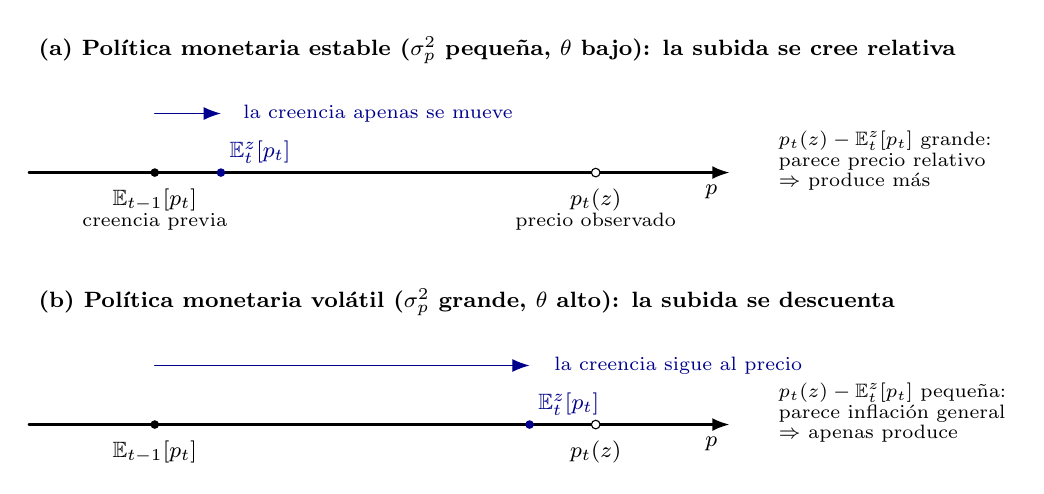
\begin{tikzpicture}[>={Latex[length=2.2mm]}, line cap=round, font=\footnotesize,
  eje/.style={->, thick},
  guia/.style={densely dashed, gray!80},
  pto/.style={circle, fill=black, inner sep=1.1pt}]
  % ---------- (a) politica estable ----------
  \node[anchor=west, font=\footnotesize\bfseries] at (0,4.75) {(a) Política monetaria estable ($\sigma^2_p$ pequeña, $\theta$ bajo): la subida se cree relativa};
  \draw[->, blue!55!black] (1.6,3.95) -- (2.44,3.95);
  \node[anchor=west, blue!55!black] at (2.6,3.95) {\scriptsize la creencia apenas se mueve};
  \draw[eje] (0,3.2) -- (8.9,3.2) node[below left=1pt]{$p$};
  \node[pto] (pr1) at (1.6,3.2) {};
  \node[below=3pt of pr1, inner sep=1pt, align=center] {$\mathbb{E}_{t-1}[p_t]$\\[-2pt]\scriptsize creencia previa};
  \node[circle, draw=black, fill=white, inner sep=1.1pt] (ob1) at (7.2,3.2) {};
  \node[below=3pt of ob1, inner sep=1pt, align=center] {$p_t(z)$\\[-2pt]\scriptsize precio observado};
  \node[pto, fill=blue!55!black] (po1) at (2.44,3.2) {};
  \node[above right=1pt of po1, inner sep=1pt, blue!55!black] {$\mathbb{E}^z_t[p_t]$};
  \node[align=left, anchor=west] at (9.4,3.35) {\scriptsize $p_t(z)-\mathbb{E}^z_t[p_t]$ grande:\\[-2pt]\scriptsize parece precio relativo\\[-2pt]\scriptsize $\Rightarrow$ produce más};
  % ---------- (b) politica volatil ----------
  \node[anchor=west, font=\footnotesize\bfseries] at (0,1.55) {(b) Política monetaria volátil ($\sigma^2_p$ grande, $\theta$ alto): la subida se descuenta};
  \draw[->, blue!55!black] (1.6,0.75) -- (6.36,0.75);
  \node[anchor=west, blue!55!black] at (6.55,0.75) {\scriptsize la creencia sigue al precio};
  \draw[eje] (0,0) -- (8.9,0) node[below left=1pt]{$p$};
  \node[pto] (pr2) at (1.6,0) {};
  \node[below=3pt of pr2, inner sep=1pt] {$\mathbb{E}_{t-1}[p_t]$};
  \node[circle, draw=black, fill=white, inner sep=1.1pt] (ob2) at (7.2,0) {};
  \node[below=3pt of ob2, inner sep=1pt] {$p_t(z)$};
  \node[pto, fill=blue!55!black] (po2) at (6.36,0) {};
  \node[above right=1pt of po2, inner sep=1pt, blue!55!black] {$\mathbb{E}^z_t[p_t]$};
  \node[align=left, anchor=west] at (9.4,0.15) {\scriptsize $p_t(z)-\mathbb{E}^z_t[p_t]$ pequeña:\\[-2pt]\scriptsize parece inflación general\\[-2pt]\scriptsize $\Rightarrow$ apenas produce};
\end{tikzpicture}
\end{document}
